\chapter{Experimental Results}

\textit{In this chapter, the  different components of the proof of concept explained in \cref{chap:method}are tested and the results shown. First, the  experimental setups are outlined. Afterwards the \ac{SHS} components outlined in \cref{chap:method} are tested individually. Hereafter the whole SHS-PF with activity recognition is treated.}

\section{Experimental Setups}
\label{sec:results-experimental setup}
In order to determine the performance of the \ac{SHS} \ac{PF} and its components, different experiments were devised. \par 

The step detection and step length estimation components are tested using a combination of data made available online under an open license and original data collected. The online data used for step detection and length estimation derive from the research upon which the individual methods are based on. The advantage of using online data is that it allows testing of techniques using the data from multiple test subjects holding a smartphone in multiple carrying modes, without having to perform extensive experiments.  \par 

The original data was collected personally, using an available smartwatch and smartphone. The step detection and step length estimation experiments for gathering original data  were performed outdoors using only a smartphone carried in the "in front, in hand" carrying mode, as in \cref{fig:experiment_carrying_position}. This was done since the location has no effect on accelerometer readings and outdoor testing allows for long straight walking distances, which are also easily measured from satellite images.\par 

For step detection, accelerometer measurements were recorded using different carrying modes while counting the number of steps. For step length estimation, known distance were walked and compared with the total distance estimated using the devised method. Further details on the experiments can be found in their respective sections, \cref{sec:results-step_detection} and \cref{sec:results-step_length_estimation}.    \par

Since orientation estimation and the whole indoor localization system are location-dependent, experiments were performed indoors. This was located at the residential property introduced in \cref{sec:method-particle_filter}. The tests consisted of walking around indoors with an android smartphone in hand and recording the \ac{IMU} signals in the phone through a dedicated android app. In addition, a smartwatch was worn around the wrist of the hand that was not holding the smartphone. This hand was used to open and close doors. The opening of doors was also indicated manually through the app on the smartphone, which had a button to record timestamps when pressed.\par 

In addition to recording \ac{IMU} data from both smartphone and smartwatch while the path was being walked, the trials were also being filmed from a breast pocket by another device. The video recordings are used to get a rough estimate of the path walked during the trial. This was done by replaying the video and pausing it at one second intervals. At the paused moments, the approximate position was manually indicating on the map of the experiment location. The map position and time elapsed since the start of the trial were recorded. The resulting trajectory can be used to give a rough performance indication of the indoor localization method. The full experimental process can be found in \cref{appendix:shs_experiment}. \par

A total of 6 successful trials were walked by one test subject, each trial trying to generate a different trajectory than the previous trials. The same person that generated the original data for the step detection and step length estimation experiments was also used for the indoor orientation and localization experiments.\par 


\section{Step Detection Performance}
\label{sec:results-step_detection}
The step detection method presented in \cref{sec:meth - step detection} is tested on both online and original data. In this section, first an overview of the relevant online data will be given, followed by several different metrics with which the performance of the step detection method from \cref{sec:meth - step detection} is evaluated. 


\subsection{Online Data}
\citet{Salvi2018} have released the raw accelerometer data used for their step detection algorithm under an open license. The raw data of the validation set consists of sampling time and three raw accelerometer axis signals. In addition, it indicates when a new step has been detected by the ground truth device. The ground truth device consisted of sensors placed in the soles of the test subject's shoes. This device could measure when the foot applied pressure to the sole of the shoe, indicating contact with the floor, hence when a step is taken. The dataset contains data of two users carrying the phones in different carrying modes. These are in an armband, back pocket, bag, front pocket, hand, and neck pouch. The device is carried in each carrying mode individually.  This dataset provides the opportunity to assess the performance of different step detection techniques, by comparing detections with the ground truth.\par

\subsection{Step Counting}

The step detection implementation outlined in \cref{sec:meth - step detection} was applied to the dataset of the researchers, the results of which can be found in  \cref{fig:sd_abs_comparison} and \cref{fig:sd_percent_comparison}. \cref{fig:sd_abs_comparison} compares the number of steps detected and actually taken, while \cref{fig:sd_percent_comparison}  shows the corresponding percentage error, where positive percent error indicates over-counting, while negative under-counting. \par 

In addition to the data made available online, original data was gathered outdoors in which a test subject walked exactly 60 steps in a straight line while having a smartphone in 3 different carrying modes, back pocket, front pocket, and in hand. Two trials per carrying mode were performed. The steps were counted manually. The percentage error from the ground truth can be seen in \cref{fig:202009291013step_counting_error_of_60_steps}.

The results using the opensource data of \citet{Salvi2018} indicate that the step detection implementation performs well for most carrying modes with many carrying modes having a percentage error close to 5\% or less. The original data shows similar results for smartphone in hand performance, with slightly larger error in the front pocket carrying mode.\par 

In both the opensource and original data, bad step detection performance in the back pocket carrying mode was found. Researchers attribute the bad detection in the back pocket to the pocket being loose and allowing the phone to rebound when a step was taken \cite{Salvi2018}. This would introduce nefarious components in the accelerometer signal, leading to false positives. \citet{Brajdic2013} encountered similar problems with this carrying position, hypothesizing that the relaxing of the gluteus maximus during locomotion could influence the acceleration trace.

	\begin{figure}[htbp]
		\centering
		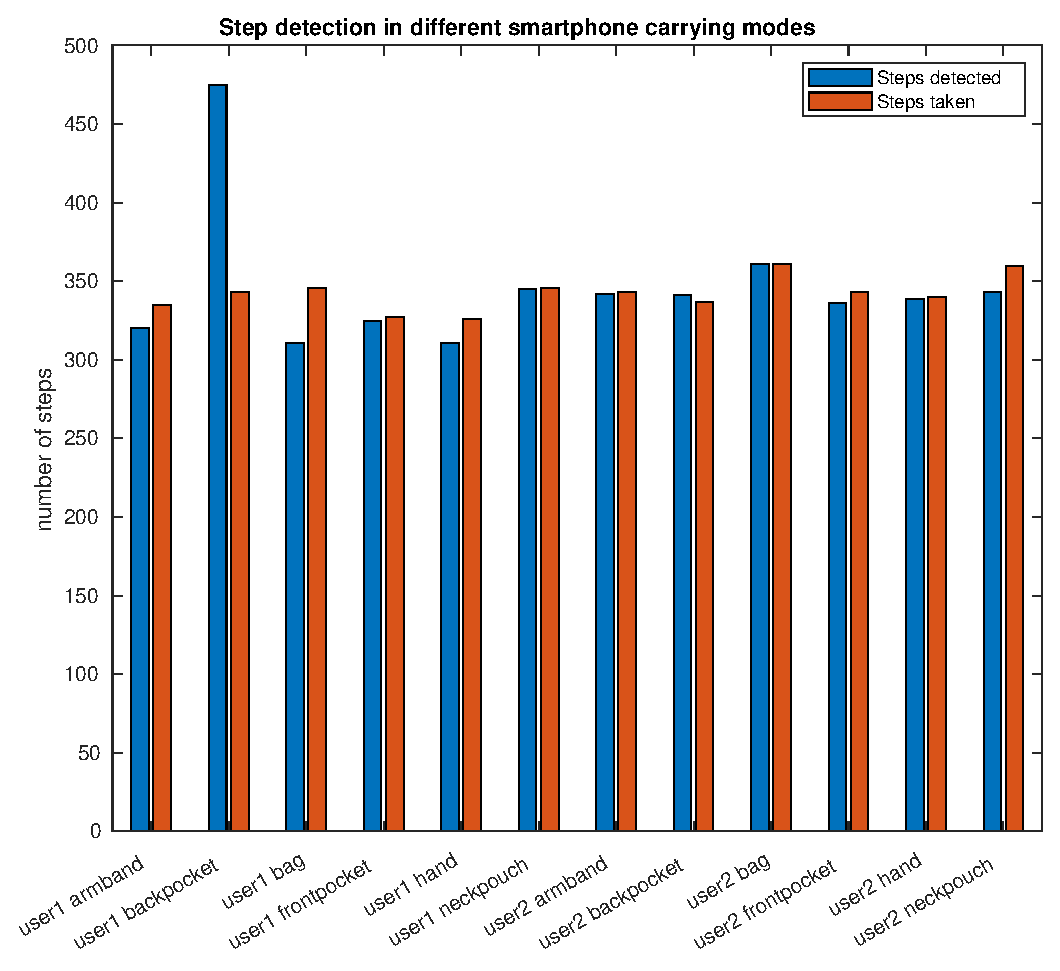
\includegraphics[width=0.7\linewidth]{images/20201127_1516_Step_detection_in_different_smartphone_carrying_modes}
		
		\caption{Absolute number of steps detected using method in \cref{sec:meth - step detection} on \citet{Brajdic2013} dataset.}
		\label{fig:sd_abs_comparison}
	\end{figure}
	\begin{figure}[H]
		\centering
		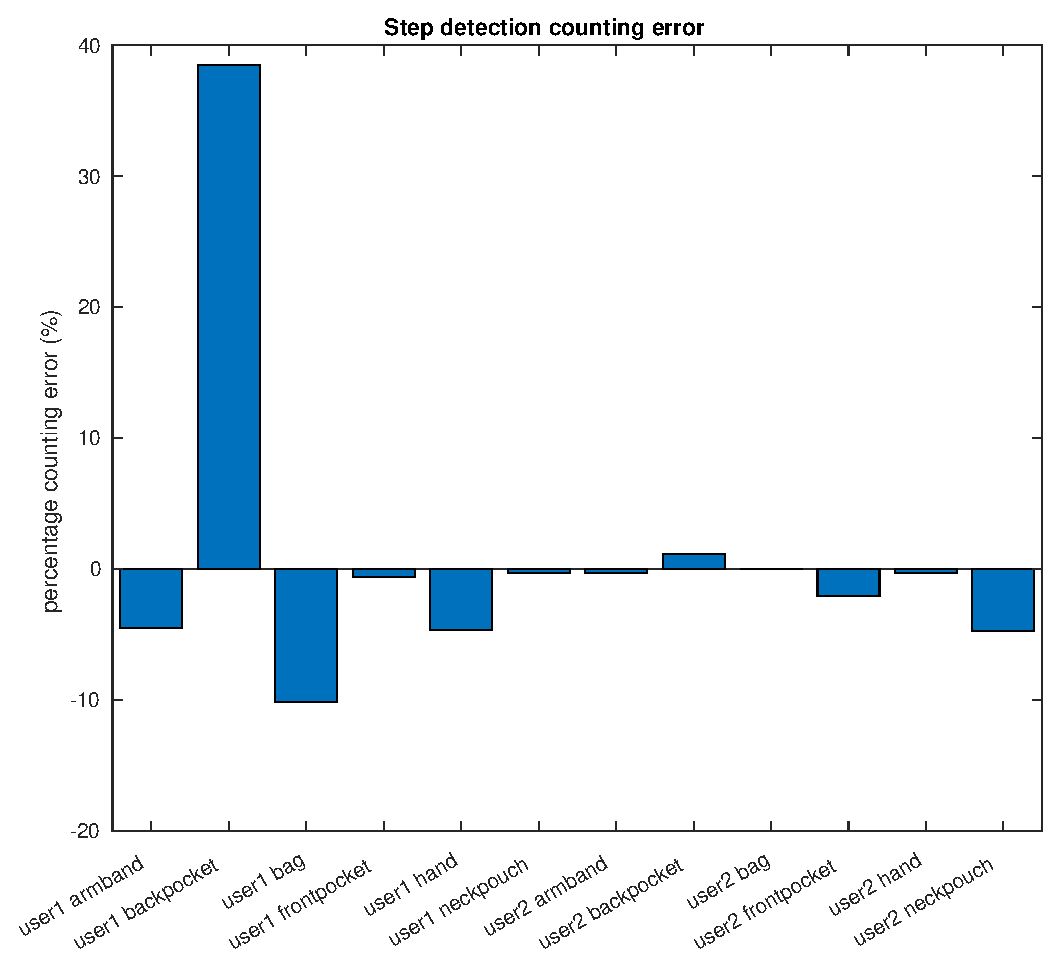
\includegraphics[width=0.7\linewidth]{images/20201127_1520_Step_detection_counting_error}
		\setlength{\belowcaptionskip}{-10pt}
		\caption{Percentage error step detections from steps taken using method in \cref{sec:meth - step detection}. }
		\label{fig:sd_percent_comparison}
	\end{figure}

%	\caption[Step detection comparison]{Comparison between \citet{Salvi2018} step detection algorithm, \cref{algo:step_detect} and ground truth for different carrying modes.}
%	\label{fig:sd_comparison}
\begin{figure}[H]
	\centering
	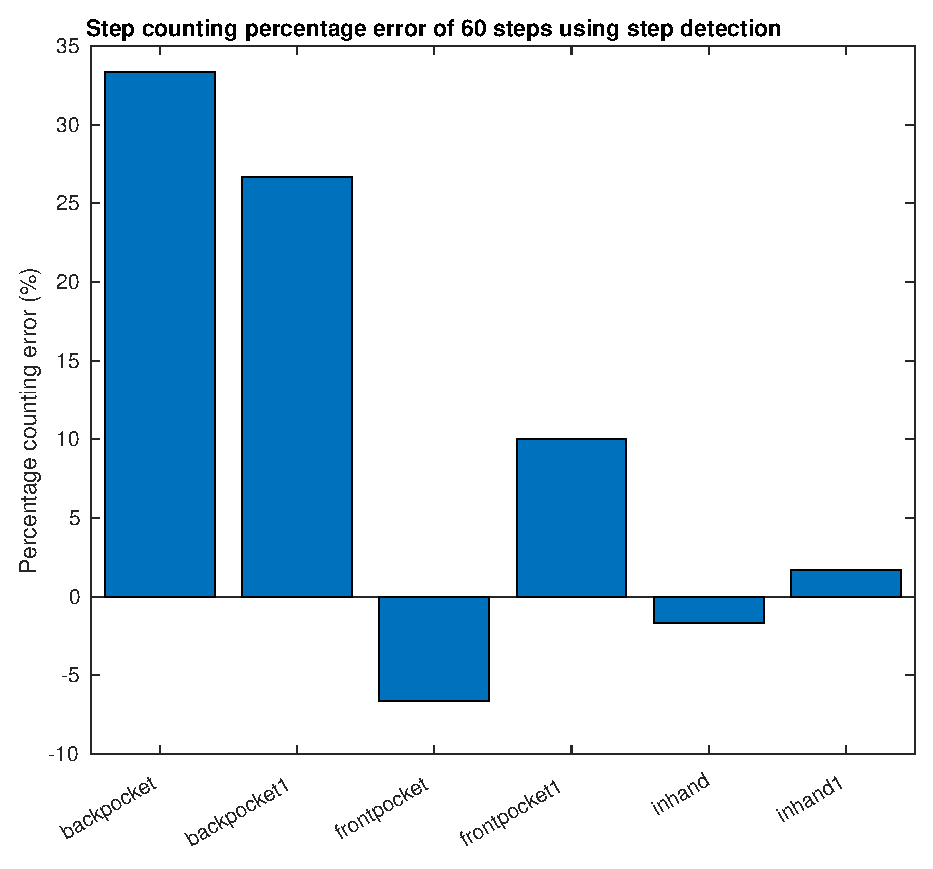
\includegraphics[width=0.7\linewidth]{images/20201127_1640_Step_counting_percentage_error_of_60_steps_using_step_detection}
	\setlength{\belowcaptionskip}{-20pt}
	\caption{Original data step counting using method in \cref{sec:meth - step detection} on \citet{Brajdic2013} dataset.}
	\label{fig:202009291013step_counting_error_of_60_steps}
\end{figure}

\subsection{Time Difference between Detection and Ground Truth Step}

For a \ac{SHS} it is not enough for the number of steps detected to be accurate, but also the time when a step actually occurs. Detecting a step, combined with the heading orientation at that moment, determines the displacement vector. It is therefore preferable for a detection to be as close as possible to when a step actually occurs, with no other detections in the vicinity. \par
Using the \citet{Salvi2018} data with ground truth step detection, the time difference between a step detection and its closest ground truth point was calculated per trial. The mean and standard deviation of the time difference for each carrying mode was calculated, shown in \cref{fig:202011130914smallest_diff_to_gt_1}. 

\begin{figure}[H]
	\centering
	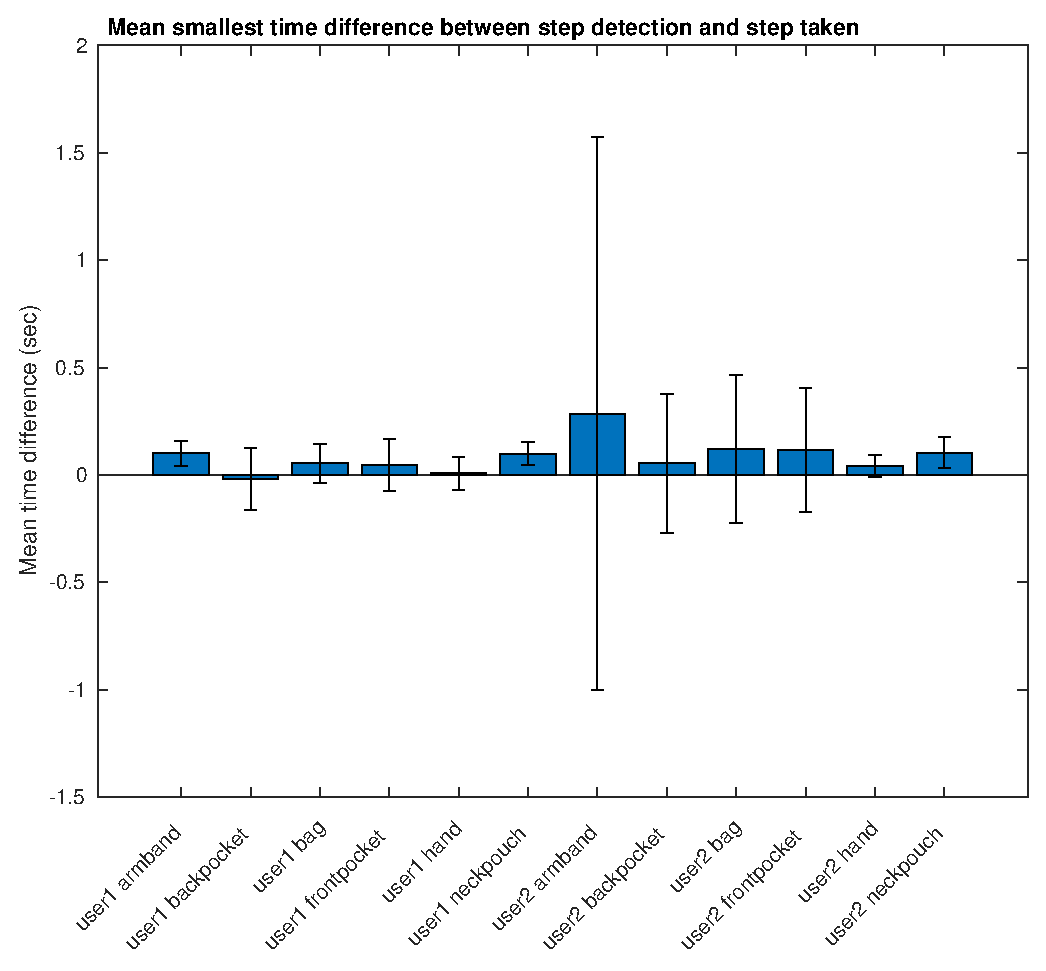
\includegraphics[width=0.7\linewidth]{images/20201127_1607_Mean_smallest_time_difference_between_step_detection_and_step_taken}
	\caption{Mean and standard deviation of the smallest time different between step detection and step occurrence using method in \cref{sec:meth - step detection} on \citet{Brajdic2013} dataset . Positive difference indicates detection before step occurrence and negative after occurrence}
	\label{fig:202011130914smallest_diff_to_gt_1}.
\end{figure}

The results show that most detections are within 0.1 seconds from the closest ground truth point. The best performing carrying mode is in hand. The large standard deviations for "user2 armband" is caused by the step detection methods having already counted multiple steps before the ground truth device has registered any. The low time difference for the backpocket carrying mode supports the hypothesis that double counting is occur close to step, since the time differences to the actual steps are small.

\subsection{Unique Step Detection}

One problem with time difference between detections and step taken is that two subsequent detections may have the same ground truth point as the nearest point, indicating that there is no unique detection of the step occurring. \par 

An approach to determining unique step detection performance was fashioned. Since it is unrealistic to expect the step detection to be at the exact time an actual step occurs, intervals are defined around ground truth step where if it is detected once within the interval using the method in \cref{sec:meth - step detection}, the detection counts as a unique step. If in this interval two steps are detected, no unique step is indicated. The time interval is increased itteratively in an attempt to find the highest unique step counts. The results for each user and carrying mode can be found in \cref{fig:sd_tp_fp_comparison}. 

\begin{figure}[H]
	\centering
	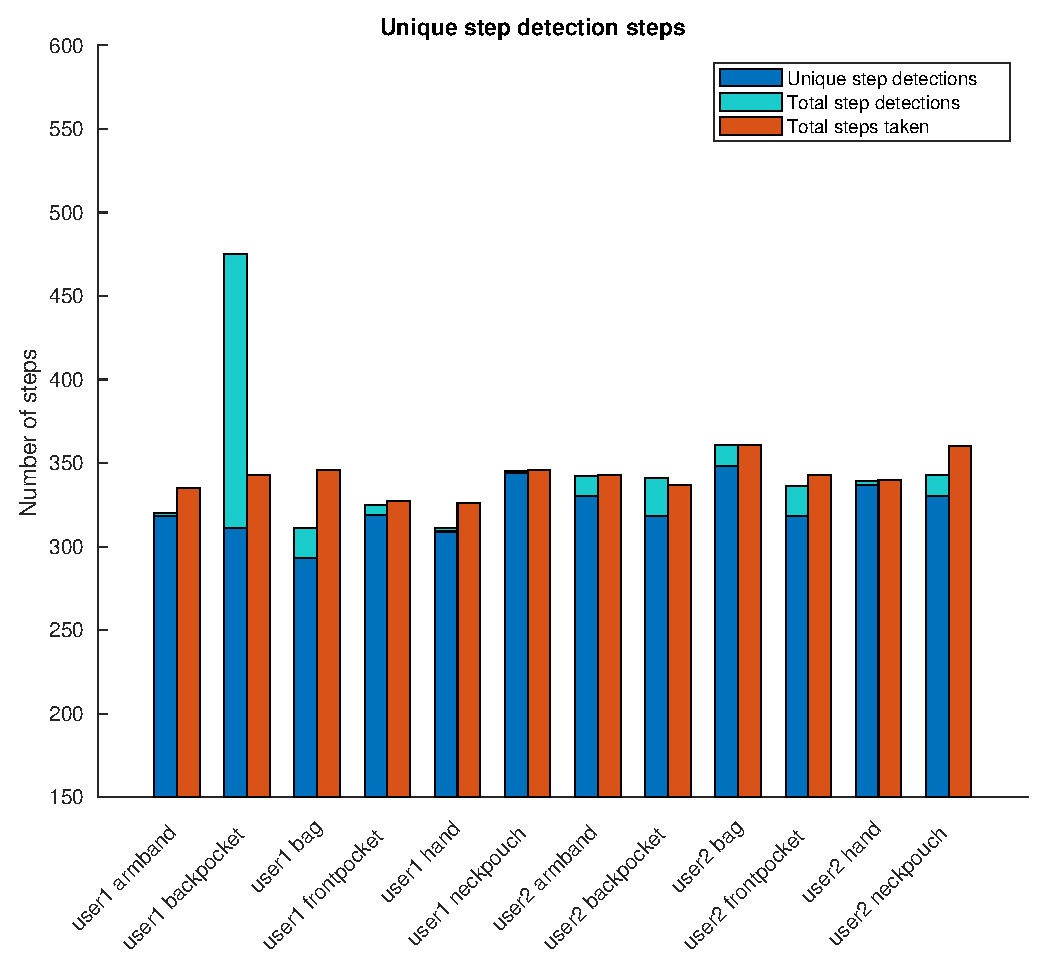
\includegraphics[width=0.7\linewidth]{images/20201127_1626_Unique_step_detection_steps}
	\setlength{\belowcaptionskip}{-10pt}
\caption[False positives and true positives step detection comparison]{Highest unique steps detected using interval method vs total number of steps taken using the method in \cref{sec:meth - step detection}. \citet{Brajdic2013} dataset is used. }
\label{fig:sd_tp_fp_comparison}
\end{figure}

These results show that the number of unique step is close to the total number of detections, indicating that the step detection method is relatively good at uniquely determining when steps are taken. \par 

From all results in step detection, the in front, in hand carrying mode has proven to be the best with low total counting error, small time difference to ground truth step and little to no double detections of the same step. This is likely caused by the fact that when held in hand, the smartphone is more or less attached to the user and has little possibility to wiggle in its constraints, in contrast to when the device is placed in pockets. It is fortunate that this carrying mode works best, since it also the carrying mode used for pedestrian heading estimation when testing the whole system.

\section{Step Length Estimation}
\label{sec:results-step_length_estimation}
For step length estimation, the linear relationships between dependent variables and step length, outlined in \cref{sec:rw - step detection} need to be determined using step detection method in \cref{sec:meth - step detection}. The step detection algorithm cannot guarantee that all steps are counted, potentially affecting the tunable parameter for both methods.  From \cref{sec:rw - step detection} the best performing algorithm for global parameters according to \cite{Vezocnik2019} is reiterated for convenience,

\begin{equation}
	\label{eq:Tian2016_sle2}
	\text{step size} = K_1 h \sqrt{F}.
\end{equation}


where $h$ is the user's height and $F$ is the step frequency. The linear relationship between step length and the dependent variables is defined by $ K_1 $, a tunable parameter. \par 

The best algorithm for individual parameters is 

\begin{equation}
	\text{step size} =K_2 \sqrt[4]{A_{\max }-A_{\min }},
	\label{eq:weinberg_stepsize2}
\end{equation}

where $A_{\max}$ and $A_{\min}$ are the maximum and minimum acceleration within a step interval. The two approaches will be used and compared to see if similar results are achieved as within \cite{Vezocnik2019}.

\citet{Vezocnik2019} have made their accelerometer data available under an open license, consists of smartphone accelerometer data of 15 different people for three walking speeds and in different carrying modes, including in front of the torso and in hand with the screen pointing up. This carrying mode will be used for step length estimation in this section, since it performed best in step detection and is used for heading estimation. \par 
Within the dataset metrics for each test subject are collected, including height, gender, and leg length. The walking speeds were defined qualitative, in that they were either slow, normal, or fast. Each person has two measurements for each walking speed, one for a 15-meter long straight path and another for a 108-meter long straight path. Within \cite{Vezocnik2019}, the smaller set is used to determine parameters for step length estimation methods, while the longer distance is used as a performance measure. This same process will be used to determine the performance of step detection and step length estimation.First the tuneable parameters $ K_1$ and $ K_2$ will be determined using the shorter length walking distances in the opensource data. \par 

\subsection{Parameter Estimation}

In \cref{fig:step_length_tian}, the dependent variables of \eqref{eq:Tian2016_sle2} are plotted against average step length. The data from the smaller distances in the \citet{Vezocnik2019} dataset are used. The average step length is calculated by dividing the distance traveled by the number of steps detected. In the figure each test subject is shown as a different color with the form of the different markers indicating the speed at which that trial was walked at. The positive upward trend indicated in \eqref{eq:Tian2016_sle2} can be observed for all test subjects as walking speed increases. In order to find the universal constant $K_1$ in \eqref{eq:Tian2016_sle2}, a linear least square estimation is performed across all test subject data points. The result is shown by the green striped line in \cref{fig:step_length_tian}, where $ K_1 = 0.3116$. \par 

A similar plot is shown in \cref{fig:step_length_weinberg}, using the same data as in \cref{fig:step_length_tian} but for the \eqref{eq:weinberg_stepsize2} dependent variables. The positive trend indicated by \eqref{eq:weinberg_stepsize2} can be noticed. Since \eqref{eq:weinberg_stepsize2} works best for personalized variable the tunable parameter $ K_2 $ is calculated per test subject, instead of all together as with \eqref{eq:Tian2016_sle2}. This is also done through the linear least square approach.

	\begin{figure}[H]
	\centering
	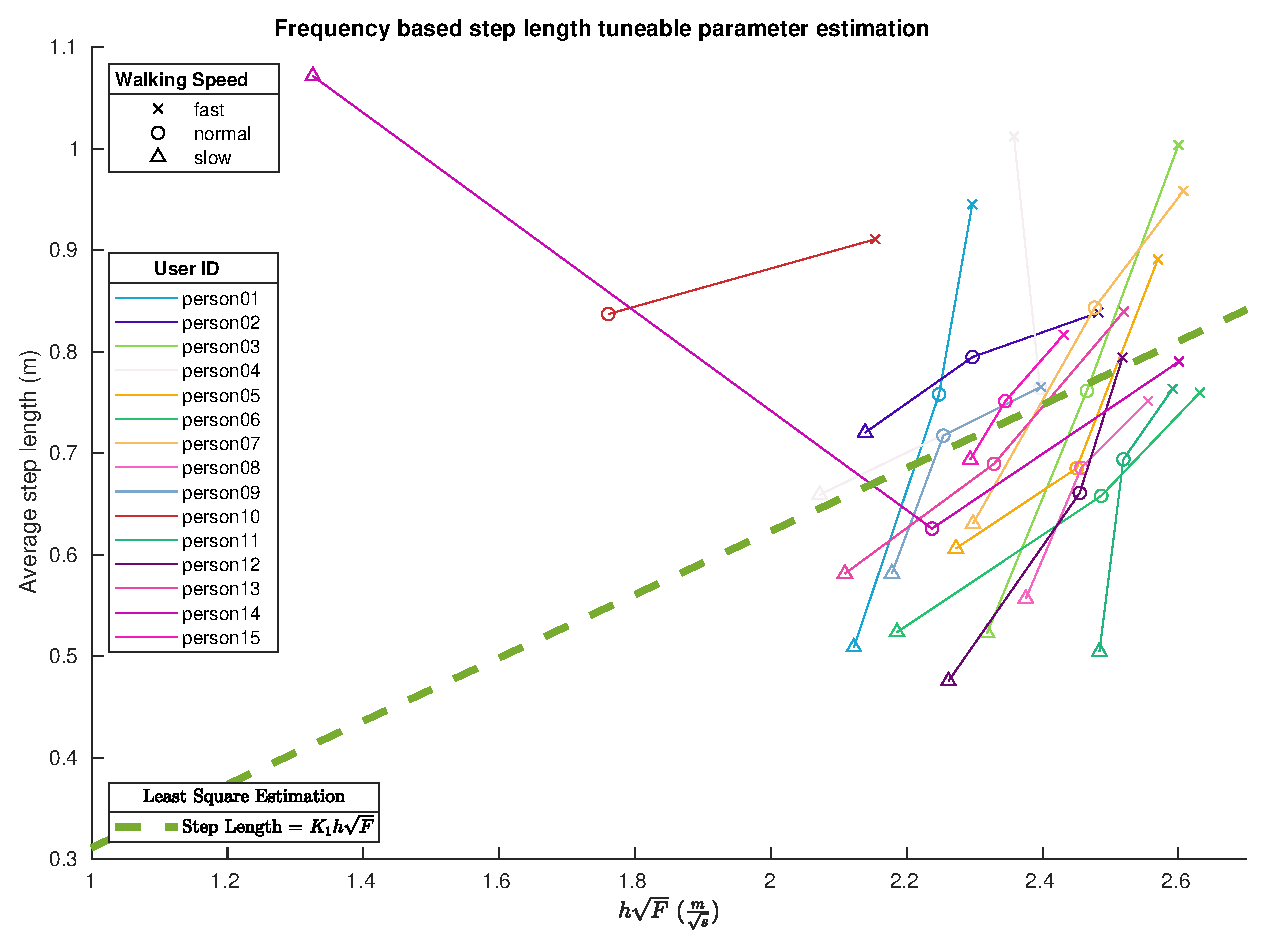
\includegraphics[width=0.8\linewidth]{images/20201128_1304_}
	\caption{Dependent variables of \eqref{eq:Tian2016_sle2} plotted against average step length over the smaller distances in the \citet{Vezocnik2019} dataset with step detection from \cref{sec:meth - step detection}. Green striped line represents \eqref{eq:Tian2016_sle2}, where $ K_1 = 0.3116$.  }
	\label{fig:step_length_tian}
	\end{figure}

\begin{figure}[h]
	\centering
	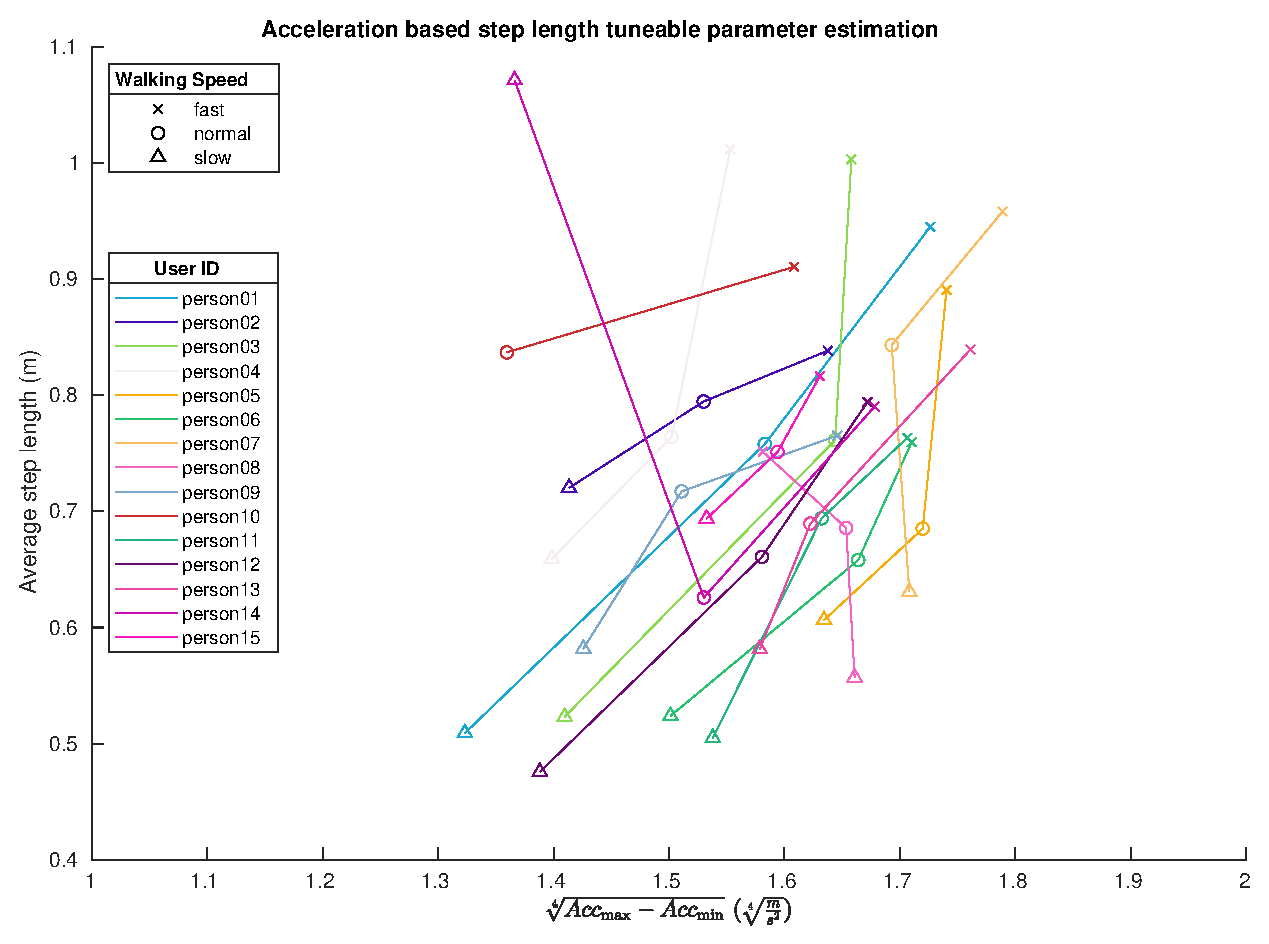
\includegraphics[width=0.8\linewidth]{images/20201128_1317_}
	\caption{Dependent variables of \eqref{eq:weinberg_stepsize2} plotted against average step length over the smaller distances in the \citet{Vezocnik2019} dataset.}
	\label{fig:step_length_weinberg}
\end{figure}

While most data seems to follow the general linear relationship for both approaches, there are two samples that do not. The two potentially faulty data points are the slow walking sample of both person 10 and 14. For the former, no steps have been detected and are therefore not visible in the plots, while for the latter too few steps have been detected. \par 

For person 14, 14 steps have been detected for slow walking, which is fewer steps than when the subject was walking fast. This is either a wrong step detection occurring, or the user walks slowly with very large steps. It is difficult to determine why this is occurring. It could be that during this sample, the test subject was holding the phone incorrectly, the person had a very different step strategy when performing at this speed, or the phone was malfunctioning. \par 

This outlier affects the eventual tunable parameter for both step length approaches. Removing it will change the estimate of $K_1$ from 0.3116 to 0.3080. The validation dataset can be used to determine if the difference in the tunable parameter has a significant effect on the total distance traveled. The difference was found to have a negligible effect on the outcome of the method.
%The results are found in  \cref{fig:step_length_estimation_validation}, where the absolute distance error for all walking speeds for all test subjects are shown, indicated by the dataset ID.
%\begin{figure}[H]
%	\centering
%	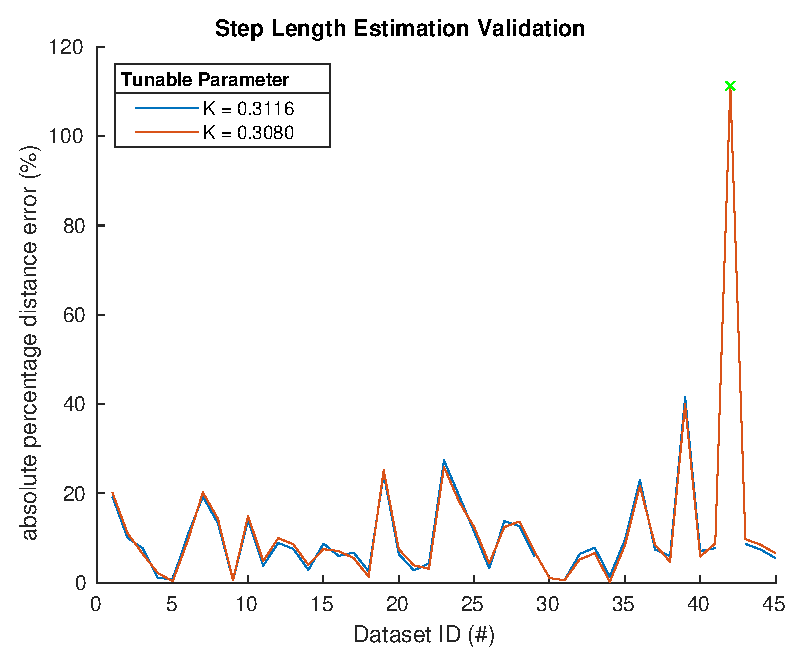
\includegraphics[width=0.65\linewidth]{images/20201028_1344_Step_Length_Estimation_Validation}
%	\setlength{\belowcaptionskip}{-30pt}
%	\caption{Step length estimation using validation dataset}
%	\label{fig:step_length_estimation_validation}
%\end{figure}

\subsection{Step Length Method Validation}

The performance of both step length estimators is evaluated by applying them to the data of the longer walking distance in the \citet{Vezocnik2019} dataset. The estimated total distance from both \eqref{eq:Tian2016_sle2} and \eqref{eq:weinberg_stepsize2} can be compared with the actual distance walked. The results are shown in  \cref{fig:202011131943_wienberg_vs_tian_vezocnik_data1}. This data surprisingly shows that depending on the test subject one or the other method is better at estimating distance traveled at different walking speeds. This does not coincide with the results of \cite{Vezocnik2019}, where \eqref{eq:weinberg_stepsize2}, which uses personalized parameters for $ K_2 $, performed better than \eqref{eq:Tian2016_sle2}, which uses general parameters for $ K_1 $. \par 

What is noticeable from the results is that there is an outlier. This is with the slow walking speed of test subject 14, which is are also the test subject with which the tunable parameter estimation had an outlier. This further supports that there is something significantly different when this test subject is performing at this walking speed.\par 

 Without the outlier, the mean absolute error for \eqref{eq:Tian2016_sle2} method is 9.7 percent with a standard deviation of 8.0 percent. For the \eqref{eq:weinberg_stepsize2} method the mean is 10.38 percent error with a standard deviation of 7.8 percent error. Both results differ from those cited by \cite{Vezocnik2019}, which indicate a mean of 7 percent with a standard deviation of 5 percent for the former and 3 percent with a 2.5 percent standard deviation for the latter.
 This is most likely caused by the difference in step detection methods, which \cite{Vezocnik2019} does not state explicitly.
 
\par

\begin{figure}[]
	\centering
	\includegraphics[width=\linewidth]{images/20201128_1403_Online_data_step_length_estimation_comparison}
	\caption{Total distance traveled estimation error from in front, in hand carrying mode from long distance data from \citet{Vezocnik2019} dataset, using \eqref{eq:Tian2016_sle2} and \eqref{eq:weinberg_stepsize2} with step detection from \cref{sec:meth - step detection}. }
	\label{fig:202011131943_wienberg_vs_tian_vezocnik_data1}
\end{figure}
 
Since no conclusive result could be distilled from applying the methods to the opensource data, a small scale experiment was performed outdoors. Within the experiment the same process as in \cite{Vezocnik2019}, where a small distance was used for parameter $ K_1 $ and $ K_2 $ estimation and a longer for performance measurement. Original data was collected from the same person and device used in the eventual indoor localization experiment. The smartphone was held in front of the torso and in hand as in \cref{fig:experiment_carrying_position}. \par 

Three trials of 30 meters were walked at different qualitative walking speeds, slow, normal, and fast, while recording accelerometer data. Four longer trials of 300 meters were walked, to determine performance, also at different walking speeds. All trials were walked with the smartphone in the same carrying mode. \par 

During the smaller walking distances, the number of steps taken was counted manually. For two trials the number of steps detected was exactly the number of steps taken. This was for slow and fast walking where 67 and 50 steps were counted respectively.  For the other trial, the detection was off 2 steps, with 57 steps being taken and 55 being recorded. With these results indicating that step detection is working properly, errors in step length estimation is likely not caused by wrongful step detection.  \par 

The different step length estimation methods were applied to the original accelerometer data. The same parameter $ K_1 $ determined for the online dataset. The $ K_2 $ parameter was based on the smaller distance data. The results are shown in \cref{fig:step_length_personal_testing}. The results suggest that for slow to normal walking step detection using \eqref{eq:Tian2016_sle2} works best, with a chance of underestimating the distance traveled. For normal to fast walking using \eqref{eq:weinberg_stepsize2} for step detection works better, with a chance of overestimating the distance traveled. By making the assumption that walking indoor is generally more in the normal to slow speed range, the choice was made to use the \eqref{eq:Tian2016_sle2} method for step length estimation in the indoor localization system.
\begin{figure}[H]
	\centering
	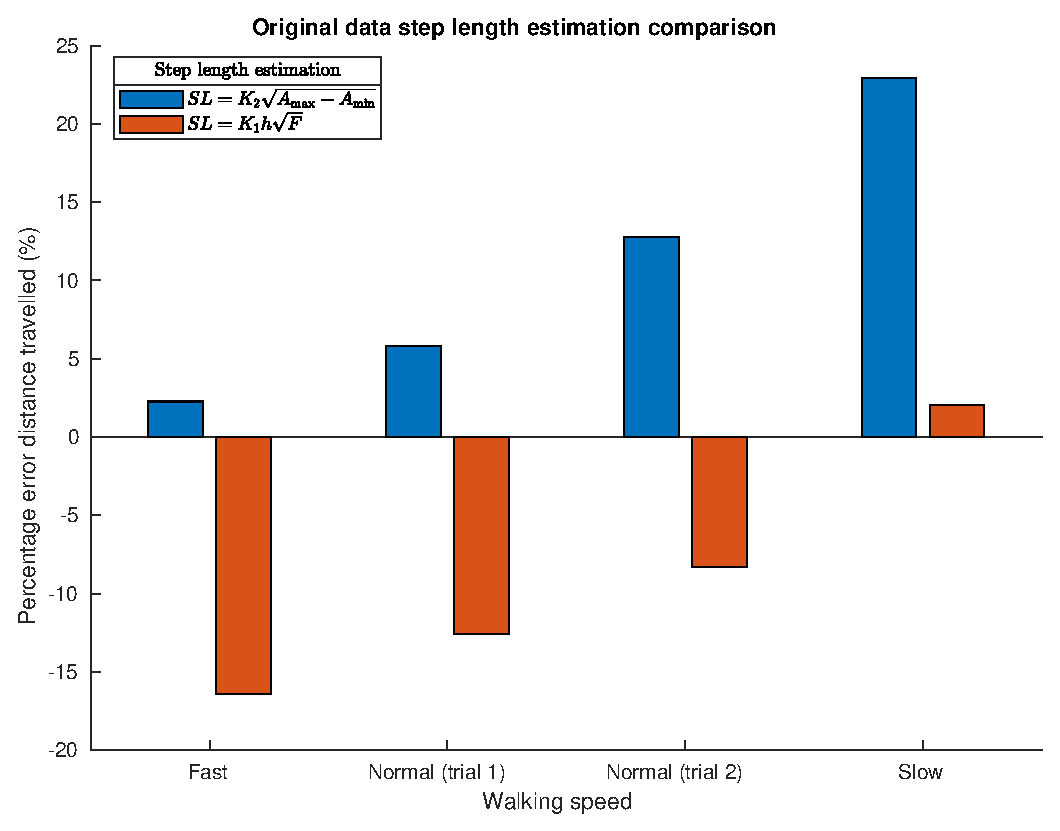
\includegraphics[width=0.7\textwidth]{images/20201128_1430_Original_data_step_length_estimation_comparison}
		\setlength{\belowcaptionskip}{-15pt}
	\caption{Step length estimation method comparison using original accelerometer data recording while walking and step detection from \cref{sec:meth - step detection}. }
	\label{fig:step_length_personal_testing}
\end{figure}

For both the opensource data and the original data the accelerometer based method in \eqref{eq:weinberg_stepsize2} does not necessarily work better than frequency based method in \eqref{eq:Tian2016_sle2}, as indicated by \citet{Vezocnik2019}. For future work it may be worthwhile to test the other algorithms outlined by \cite{Vezocnik2019} to see if there are any other differences between the outcomes. 

\section{Indoor Orientation Estimation}

Determining the performance of orientation estimation during the indoor experiments is difficult since no ground truth was available for comparison. A sanity check that can be performed is comparing the orientation estimations of the EKF with the orientation estimations calculated by the android operating system. The results will not be able to give an indication of which performed best with respect to reality, but could potentially highlight any very diverging behavior. \par 

In order to calculate an orientation difference, a difference quaternion ($	\Delta q_t$) can be used, defined as \cite{Kok2017}

\begin{equation}
	\Delta q_t = \hat{q}_{t}^{nb} \odot \left( \hat{q}_{comp,t}^{nb}  \right)^c,
\end{equation} 

where $\hat{q}_{comp,t}^{nb}$ is the unit quaternion that $ \hat{q}_{t}^{nb} $ is compared with.  In order to compare the orientation estimates of the android system and the EKF from \cref{algo:indoor_EKF}, the difference in angle between the first quaternion estimate and the following quaternions estimate is calculate for both orientation estimates. This is done to calculate the relative orientation estimate to the initial orientation, which are the angles used by the \ac{SHS}.\par 

Since both relative orientation estimates start at the same initial quaternion, the two estimates can now be compared. Applying the difference quaternion calculation to these estimates, the difference quaternions over the whole orientation estimate are determined.  \par 

Once calculated, the difference quaternions can be converted into Euler angles for more intuitive interpretation. The mean difference in yaw component for each trial is shown in  \cref{fig:yaw_difference_between_android_and_ekf_1}. From the results, the difference between both orientation estimations seems larger for trial 3 and 6, requiring further investigation.

\begin{figure}[H]
	\centering
	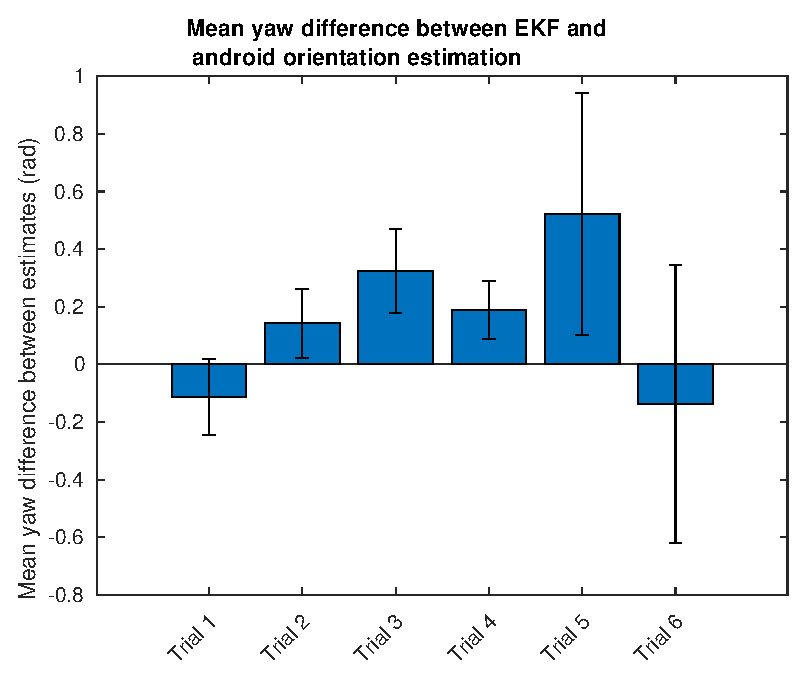
\includegraphics[width=0.7\linewidth]{images/20201128_1646_mean_yaw_difference_1}
	\setlength{\belowcaptionskip}{-20pt}
	\caption{Mean yaw difference between \cref{algo:indoor_EKF} and android orientation estimates.}
	\label{fig:yaw_difference_between_android_and_ekf_1}
\end{figure}

\newpage
\section{Step and Heading System Particle Filter Testing}

Through the indoor experiment outlined in \cref{sec:results-experimental setup} the complete indoor localization system could be tested from input sensor measurements and map information to postion estimate. The IMU data is passed through the \ac{SHS} subsystem of \cref{sec:method-SHS} to produce a \ac{SHS} trajectory. The smartwatch IMU data is passed through the activity recognition method in \cref{sec:method-AR} to  detect door interaction. Combining the \ac{SHS} trajectory and door interaction detection with the floor map generated in \cref{sec:method-particle_filter}, the Particle Filter propagates position estimates through the indoor environment, while taking spatial context into account. The resulting trajectories from the particles at the last time step of the SHS are averaged to produce the indoor position estimate over the experiment , as explained in \cref{sec:method-pf_location_estimate}. The whole system combined will be referred to as the Step and Heading Particle Filter (SHS-PF).  \par 

By using the video recordings made during the different trials, a rough position trajectory was created. This rough estimate can be used for comparison with the position estimate of the \ac{SHS} Particle Filter, in order to get an indication of the estimating performance. This can be done by calculating the root-mean-square error between the two position estimate as

\begin{equation}
	\displaystyle \operatorname {RMSE} ={\sqrt {\frac {\sum _{t=1}^{T}({\hat {y}}_{t}-y_{t})^{2}}{T}}},
	\label{eq:RMSE}
\end{equation}

where $T$ is the total time of the trial, $\hat{y_t}$ the postion estimate at time $t$ of the SHS-PF and $y_t$ the video trajectory position at time $t$.

\subsection{SHS-PF with Manually Labeled Door Interaction}
\label{sec:results-SHS_PF_manually indicated}
During the experiment, timestamps were recorded to indicate the beginning of interaction with a door within the indoor environment. The recorded timestamps can be used to trigger a Particle Filter door interaction measurement update. Using this method, the potential effect of activity recognition for indoor localization in the ideal case can be evaluated, since there is no chance for false positives to occur.\par

This section will first use these additional position measurements to find model parameters, through an iterative process. First the number of particles to use will be estimated. Afterwards the standard deviations in the time update of the Particle Filter will be determined. Once these parameters are defined, the performance of SHS-PF with manually labeled door interaction is evaluated.

\subsubsection{Determining Particle Filter Time Update Standard Deviations}

\subsubsection{Determining Number of Particles}

This represent particle runs that have been able to propagate particles for the whole \ac{SHS} trajectory.
 
\begin{figure}[H]
	\centering
	\begin{subfigure}[t]{.38\textwidth}
		\centering
		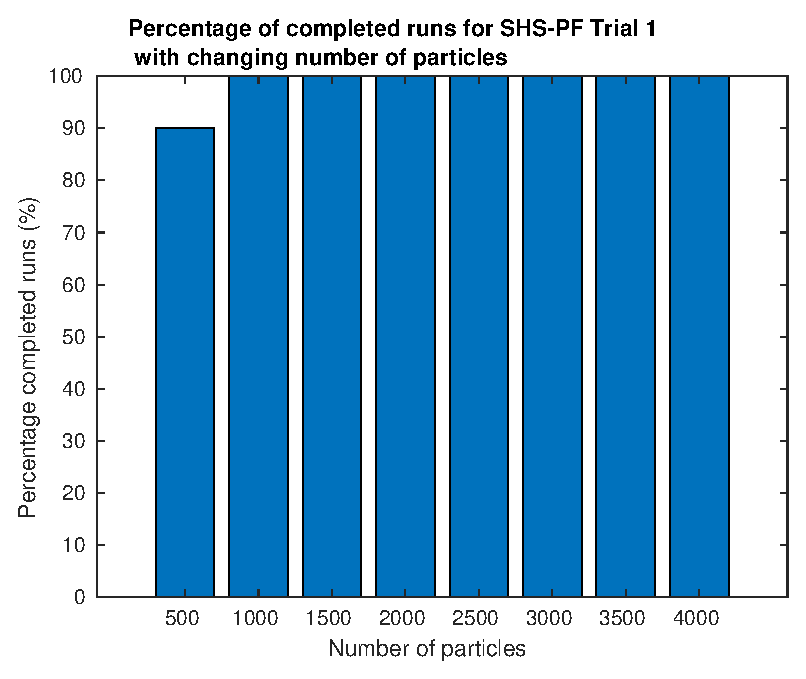
\includegraphics[width=\linewidth]{images/20201129_1147_Trial_1_nr_particles_1}
		\caption{}
		\label{fig:trial1_nr_particles}
	\end{subfigure} \quad
	\begin{subfigure}[t]{.4\textwidth}
		\centering
		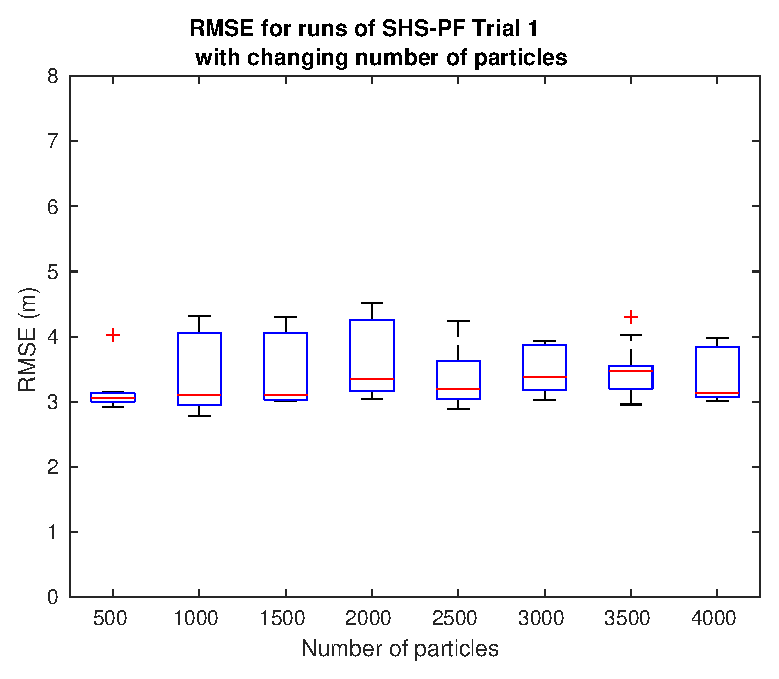
\includegraphics[width=\linewidth]{images/20201129_1154_Trial_1_RMSE_nr_particles_1}
		\caption{}
		\label{fig:trial3_nr_particles}
	\end{subfigure} \quad
\end{figure}

\begin{figure}[H]
	\centering
	\begin{subfigure}[t]{.4\textwidth}
		\centering
		\includegraphics[width=\linewidth]{images/20201129_1147_Trial_3_nr_particles_1}
		\caption{}
		\label{fig:trial3_nr_particles}
	\end{subfigure} \quad
\begin{subfigure}[t]{.4\textwidth}
	\centering
	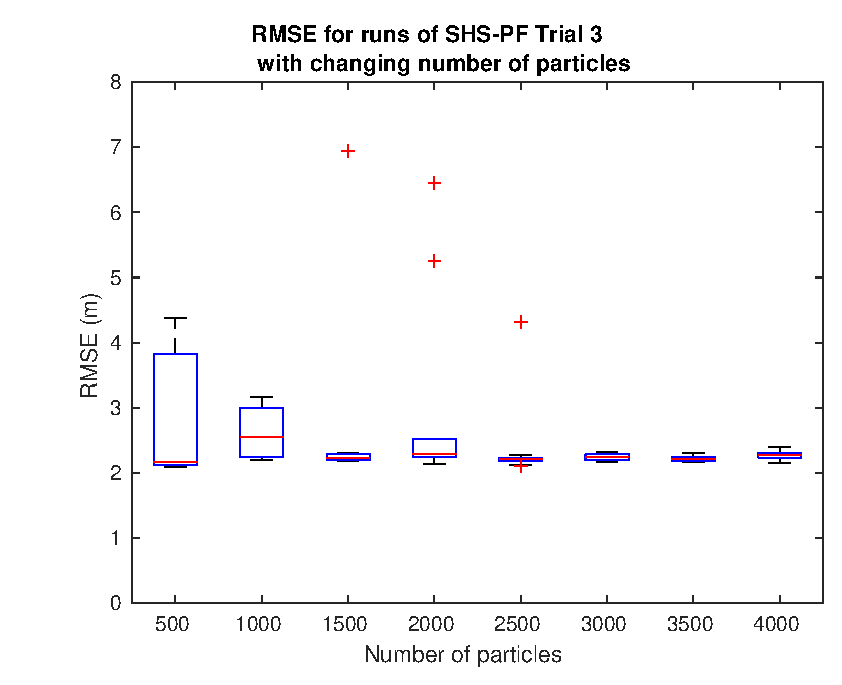
\includegraphics[width=\linewidth]{images/20201129_1154_Trial_3_RMSE_nr_particles_1}
	\caption{}
	\label{fig:trial3_nr_particles}
\end{subfigure} \quad
\end{figure}

\subsubsection{Performance}
All trials were run through the complete SHS-PF with the manually recorded door interactions, with 4000 particles. This was done for five runs per trial, in order to show reproducibility. The results can be found in \cref{fig:pf_boxplot}. The figure shows the root-mean-square errors values per experimental trial over 5 runs. At the top of the figure the amount of completed runs is indicated.

\begin{figure}[H]
	\centering
	\includegraphics[width=0.7\textwidth]{images/20201129_1419_RMSE_manually_indicated_ar_shspf_trials_1}
	\caption[Particle Filter position estimation performance with manual door interaction]{Particle Filter position estimation root mean square error compared to rough video generated estimate. Manually indicated door interactions were used for Particle Filter measurement update.}	
	\label{fig:pf_boxplot}
\end{figure}

The results show that for trials 1 to 3 and trial 6 that all five runs were completed, with their individual runs having similar RMSE values to the rough video estimate. The RMSE value per trial do vary, which can be explained by looking at the trajectory that the system generates. \par  

While the particles for trial 1 and 2 complete all iterations, however both do not follow the complete trajectory derived from video analysis. This can be seen in  \cref{fig:shspf_trial1_shs_gt_comparison} where the structure circled in green is circled by the rough estimate but not by the Particle Filter. For \cref{fig:shspf_trial2_shs_gt_comparison} the Particle Filter seems to walk too far and is unable to make the correct turn.

\begin{figure}[H]
	\centering
	\begin{subfigure}[t]{.45\textwidth}
		\centering
		\begin{tikzpicture}
			\node[anchor=south west,inner sep=0] (image) at (0,0) {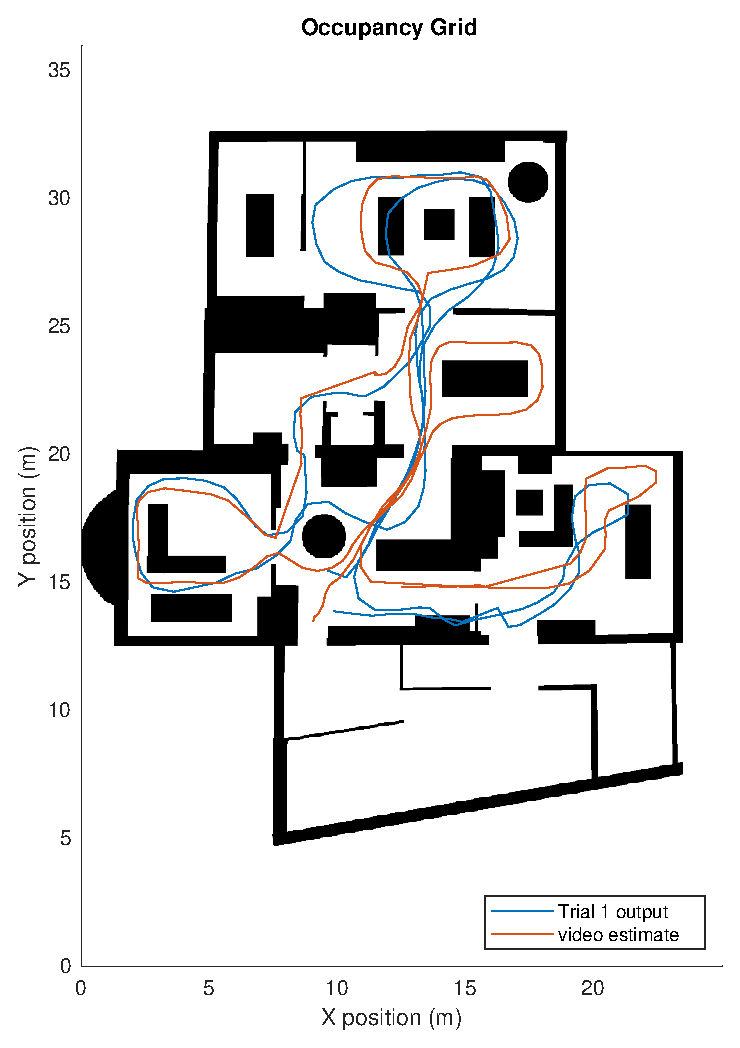
\includegraphics[width=0.9\textwidth]{images/20201118_1900_trial1_output_2}};
			\begin{scope}[x={(image.south east)},y={(image.north west)}]
				\draw[green,ultra thick,rounded corners] (0.6,0.625) rectangle (0.73,0.66);
			\end{scope}
		\end{tikzpicture}		
		\caption{trajectory comparison}
		\label{fig:shspf_trial1_on_map}
	\end{subfigure}
	\begin{subfigure}[t]{.45\textwidth}
		\centering
		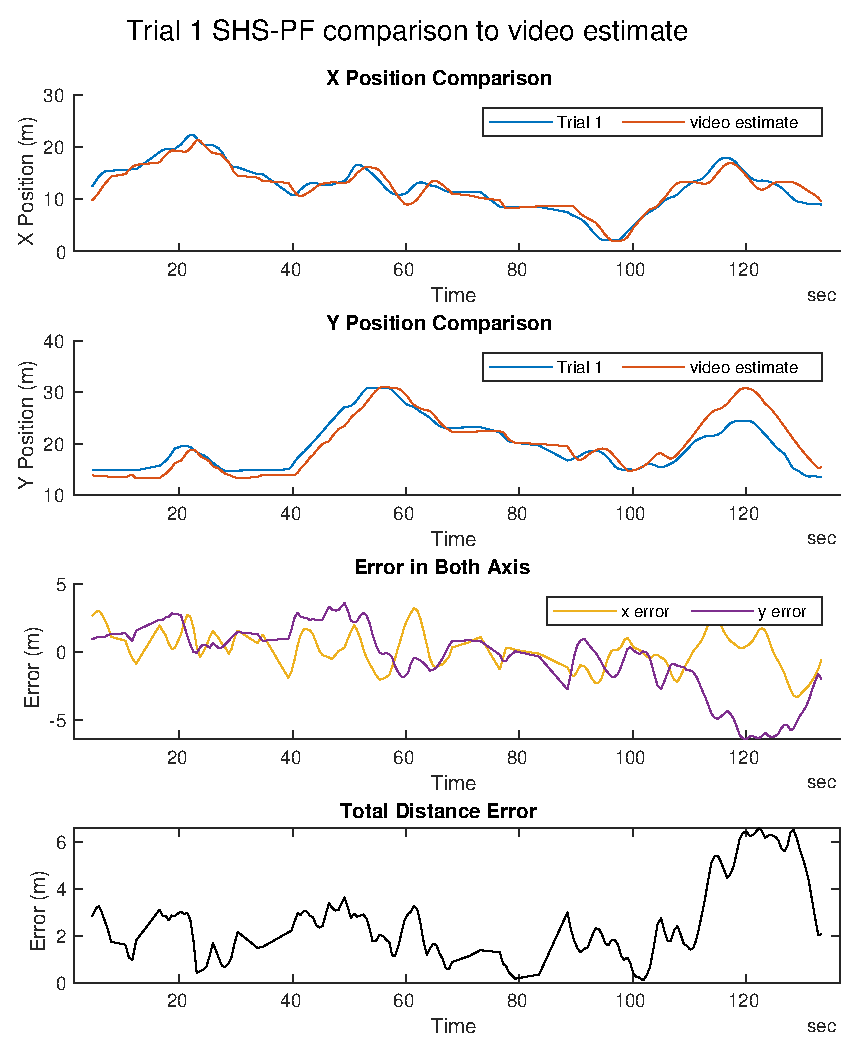
\includegraphics[width=\linewidth]{images/20201118_1900_trial1_output_1}
		\caption{axis comparison}
		\label{fig:shspf_trial1_comparison}
	\end{subfigure}
	\setlength{\belowcaptionskip}{-20pt}
	\caption{SHS-PF comparison of trial 1 with ground truth}
	\label{fig:shspf_trial1_shs_gt_comparison}
\end{figure}
\begin{figure}[H]
	\centering
	\begin{subfigure}[t]{.45\textwidth}
		\centering
		\includegraphics[width=0.9\linewidth]{images/20201118_1902_trial2_output_2}
		\caption{trajectory comparison}
		\label{fig:shspf_trial2_on_map}
	\end{subfigure}
	\begin{subfigure}[t]{.45\textwidth}
		\centering
		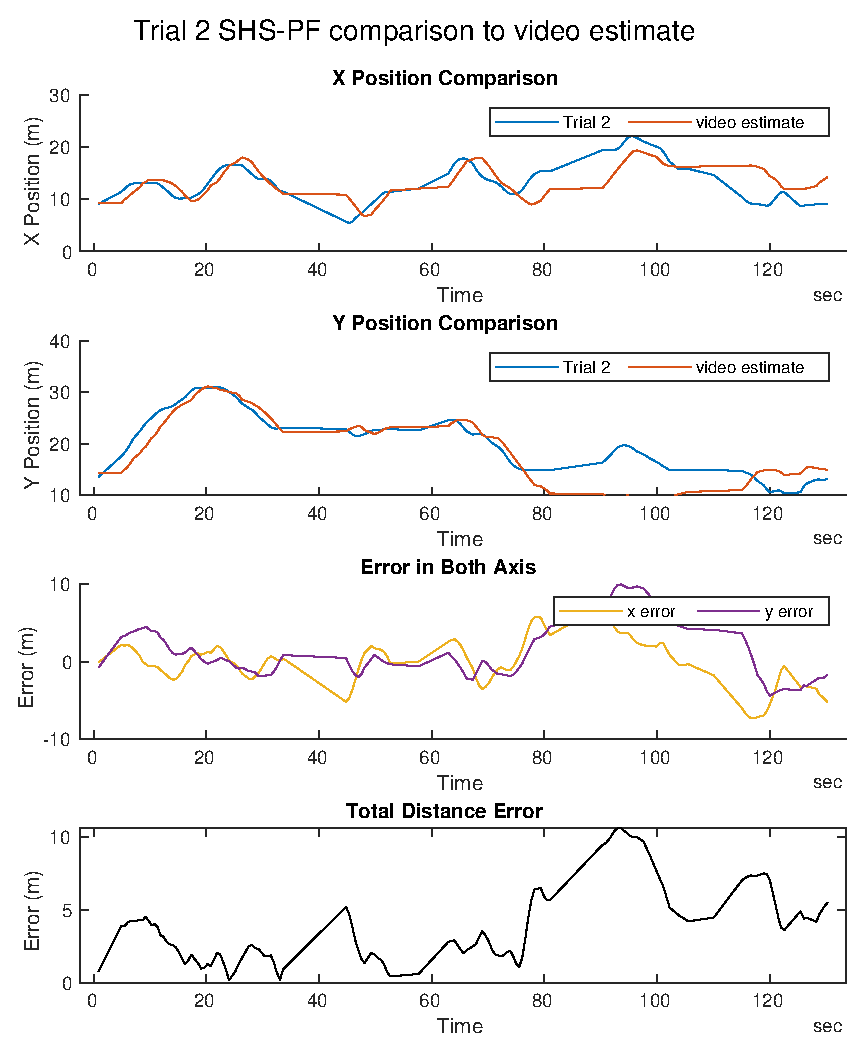
\includegraphics[width=\linewidth]{images/20201118_1902_trial2_output_1}
		\caption{axis comparison}
		\label{fig:shspf_trial2_comparison}
	\end{subfigure}
	\caption{SHS-PF comparison of trial 2 with ground truth}
	\label{fig:shspf_trial2_shs_gt_comparison}
\end{figure}

 Trial 3 and 7 are able to follow the route better. corresponding to lower RMSE values, the outputs are shown in \cref{fig:shspf_trial7_shs_gt_comparison}.
I have a hypothesis that step length estimation is overestimating distance traveled in some cases. This can be caused by turning not having the same displacement as a straight step.
Show a table of the distance walked according to rough video estimate and what the \ac{SHS}estimated.

Trials 5 and 6 are unable to complete any iteration reliably even with "perfect" activity recognition. This seems to suggest that the output of the \ac{SHS}is not good enough. This needs to be shown in figures.


The total SHS-PF solution was unable to get a reliable output for trials 4 and 5.\par 

\subsection{SHS- PF with Door Interaction Detection}
Applying the activity recognition method on the smartwatch data outline in Algorithm 3, door interactions could be detected. Using these detections instead of the manually indicated ones, the results in \cref{fig:rmse_per_trial_with_activity_recognition} were generated

\begin{figure}[H]
	\centering
	\includegraphics[width=0.7\linewidth]{images/RMSE_door_interaction_detections_ar_shspf_trials}
	\caption[Particle Filter position estimation performance with door interaction]{Particle filter position estimation root mean square error compared to rough video generated estimate using detected door interactions.}
	\label{fig:rmse_per_trial_with_activity_recognition}
\end{figure}

Trials 1,2 and 6 show similar results as when "perfect" activity recognition was used. Also the inability to complete all iterations for trials 5 and 6 is still present. In contrast trial 3 is also unable to complete all iterations, with the completed iterations leading to much larger RMSE values than before. 

\subsection{SHS-PF without Door Interaction Measurement Update}
In order to see what effect activity recognition measurement updates have on estimating the trajectory, the Particle Filter needs to be run without them. All other parameters were kept the same. The results can be found in \cref{fig:pf_boxplot_no_doors}.

\begin{figure}[H]
	\centering
	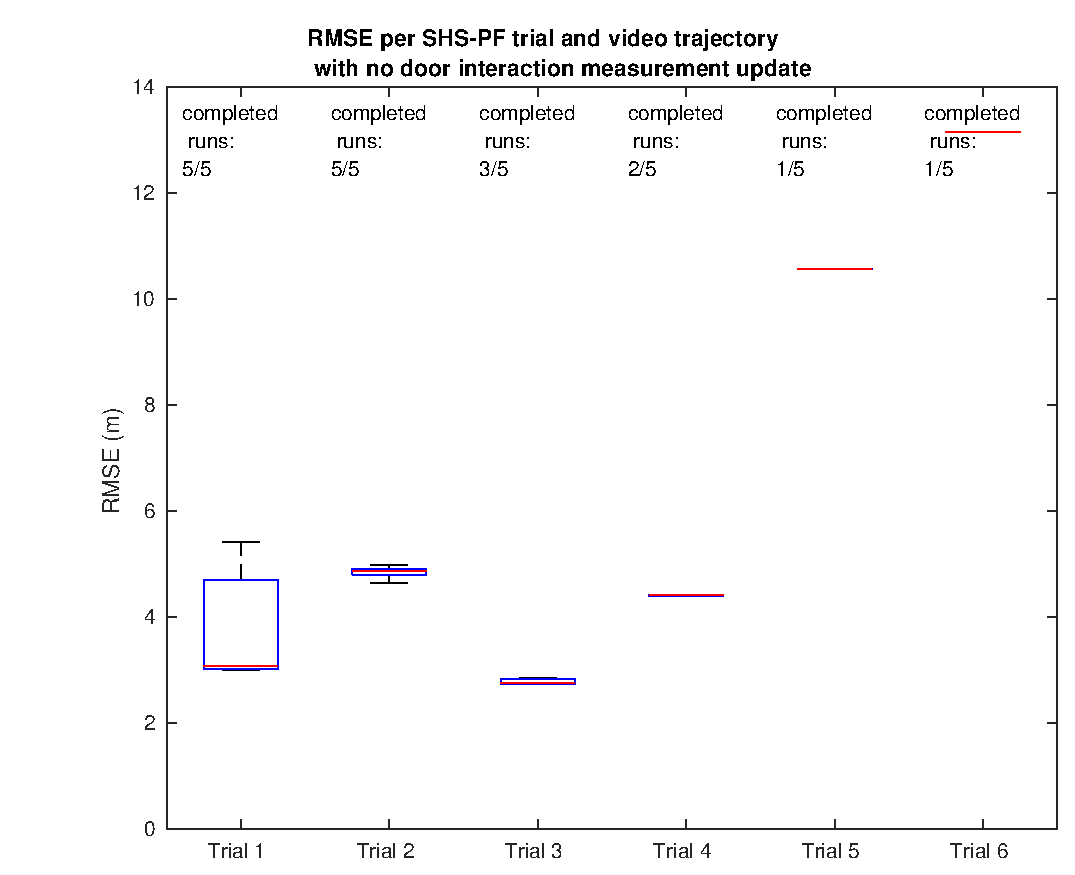
\includegraphics[width=0.7\textwidth]{images/20201129_1438_RMSE_with_no_door_interaction_1}
	\caption[Particle Filter position estimation performance without door interaction]{Particle Filter position estimation performance without door interaction measurement update, 5 iterations per trial. Number under "completed" indicates how many iteration had particles surviving for the whole \ac{SHS}trajectory.}
	\label{fig:pf_boxplot_no_doors}
\end{figure}

The results show that trials 3, and 5 to 7 were unable to complete all iterations. Trial 2 seems to have no difference in performance compared to when activity recognition is used. The RMSE value for trial 1 is similar to that when activity recognition is used, while the spread is larger.